\chapter{Results and Discussion}
\label{chapter: 6}

This chapter outlines how results are obtained from the system and uses these results to discuss how successful the project was. Ideas for future work related to the project are included as well. 

\section{Results}

In order to evaluate the performance of the system after it has finished, some data is recorded. On every tick a new record is saved, containing data points for useful information such as estimated ball position and velocity. As well as this, data is stored for each accepted ball candidate including the candidate's image and world position. The tests described in the following sections will be performed using this data. 

The system will be run through a set of six scenarios to test the performance in various situations, shown in figure \ref{fig: scenarios}. The first three tests contain only the MiRo and the ball, with the ball moving across the MiRo, away from it and towards it respectively. The last three tests use the same ball motion, but include another MiRo to interfere with the perception system. In scenarios 4 and 6 the ball passes in front of the other MiRo, and passes behind in scenario 5, obscured vision for a period of time. The tests will be run in simulation as this allows the real position of the ball to easily be recorded, and the tests can be easily repeated. To get a robust average of results the test will be repeated 20 times. 

\begin{figure}[H]
    \begin{tikzpicture} 
    \begin{axis} [
        ymin=-1.3,
        ymax=1.3,
        xmin=-1.95,
        xmax=1.95,
        xlabel=Scenario 1
    ]
    \addplot [only marks] table {
0 0
};
\addplot [only marks, mark=o] table {
1 -1
1 1.15
};
\draw[->] (axis cs:1,-1) -- (axis cs:1,1.15);
    \end{axis} 
    \end{tikzpicture}
%
\begin{tikzpicture} 
    \begin{axis} [
        ymin=-1.3,
        ymax=1.3,
        xmin=-1.95,
        xmax=1.95,
        xlabel=Scenario 2
    ]
    \addplot [only marks] table {
0 0
};
\addplot [only marks, mark=o] table {
0 1
1.5 0.35
};
\draw[->] (axis cs:0,1) -- (axis cs:1.5,0.35);
    \end{axis} 
\end{tikzpicture}

\begin{tikzpicture} 
    \begin{axis} [
        ymin=-1.3,
        ymax=1.3,
        xmin=-1.95,
        xmax=1.95,
        xlabel=Scenario 3
    ]
    \addplot [only marks] table {
0 0
};
\addplot [only marks, mark=o] table {
1.5 0.5
-0.3 -0.725
};
\draw[->] (axis cs:1.5,0.5) -- (axis cs:-0.3,-0.725);
    \end{axis} 
\end{tikzpicture}
%
    \begin{tikzpicture} 
    \begin{axis} [
        ymin=-1.3,
        ymax=1.3,
        xmin=-1.95,
        xmax=1.95,
        xlabel=Scenario 4
    ]
    \addplot [only marks] table {
0 0
};
\addplot [only marks, mark=o] table {
1 -1
1 1.15
};
\addplot [only marks, mark=triangle] table {
1.5 0.2
};
\draw[->] (axis cs:1,-1) -- (axis cs:1,1.15);
    \end{axis} 
    \end{tikzpicture}

\begin{tikzpicture} 
    \begin{axis} [
        ymin=-1.3,
        ymax=1.3,
        xmin=-1.95,
        xmax=1.95,
        xlabel=Scenario 5
    ]
    \addplot [only marks] table {
0 0
};
\addplot [only marks, mark=o] table {
0 1
1.5 0.35
};
\addplot [only marks, mark=triangle] table {
0.5 0.5
};
\draw[->] (axis cs:0,1) -- (axis cs:1.5,0.35);
    \end{axis} 
\end{tikzpicture}
%
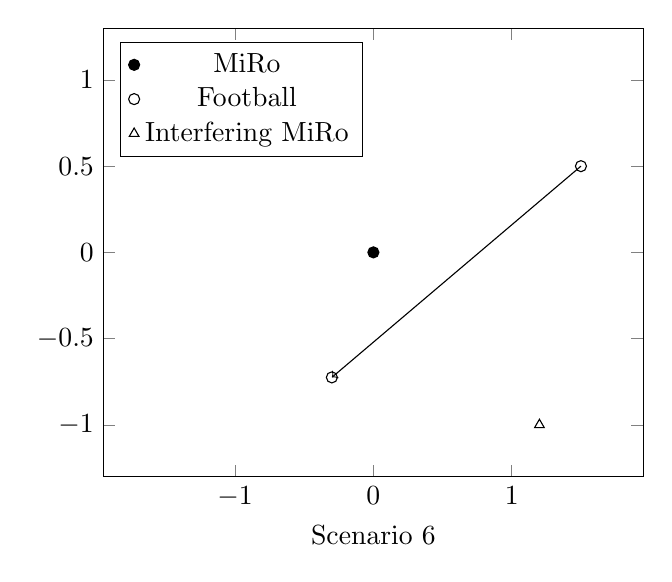
\begin{tikzpicture} 
    \begin{axis} [
        ymin=-1.3,
        ymax=1.3,
        xmin=-1.95,
        xmax=1.95,
        xlabel=Scenario 6,
        legend style={at={(0.03,0.97)},anchor=north west}
    ]
    \addplot [only marks] table {
0 0
};
\addlegendentry{MiRo}
\addplot [only marks, mark=o] table {
1.5 0.5
-0.3 -0.725
};
\addlegendentry{Football}
\addplot [only marks, mark=triangle] table {
1.2 -1
};
\addlegendentry{Interfering MiRo}
\draw[->] (axis cs:1.5,0.5) -- (axis cs:-0.3,-0.725); 
    \end{axis} 
\end{tikzpicture}
\caption{Scenarios used to evaluate the system}
\label{fig: scenarios}
\end{figure}

\subsection{Ball Position}

\subsubsection{Relative Error}

The primary metric for the accuracy of the ball position estimation uses relative error. This is preferred over absolute error as it is more lenient when the ball is far away, and more strict when the ball is close. The relative error is used to calculate an overall score as a percentage, where 100\% is perfect accuracy and 0\% is infinitely inaccurate. 

\[ \text{Absolute error: } \epsilon =  |v - v_{estimate}|\]
\[ \text{Relative error: } \eta =  |1 - \frac{v_{estimate}}{v}|\]
\[ \text{Overall score: } s = \frac{1}{e^{\eta}} \]
Where $v$ is a value and $v_{estimate}$ is the estimated value.

\begin{figure}[H]
    \centering
    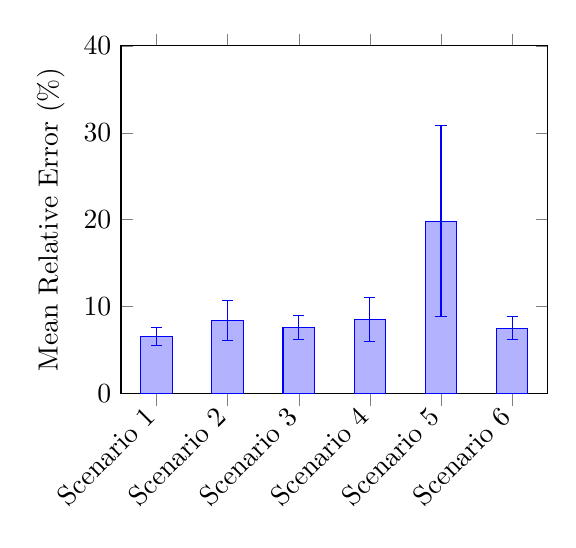
\begin{tikzpicture}
 
    \begin{axis} [ybar,
        height=6cm,
        width=7cm,
        bar width=0.4cm, 
        xlabel={}, 
        ylabel={Mean Relative Error (\%)},
        xtick={1,2,3,4,5,6},
        ymin=0,
        ymax=40,
        xticklabels={Scenario 1,Scenario 2,Scenario 3,Scenario 4,Scenario 5,Scenario 6},
        xlabel style={yshift=-1cm},
            x tick label style={
                rotate=45,
                anchor=east,
            }
        ]
     
     \addplot+ [
            error bars/.cd,
                y dir=both,
                y explicit relative,
        ] coordinates {
            (1,6.585) +- (0,0.04095*4)
            (2,8.413) +- (0,0.06813*4)
            (3,7.629) +- (0,0.04601*4)
            (4,8.514) +- (0,0.07422*4)
            (5,19.840) +- (0,0.13862*4)
            (6,7.536) +- (0,0.04379*4)
        };
     
    \end{axis}
 
    \end{tikzpicture}
    \hfill
    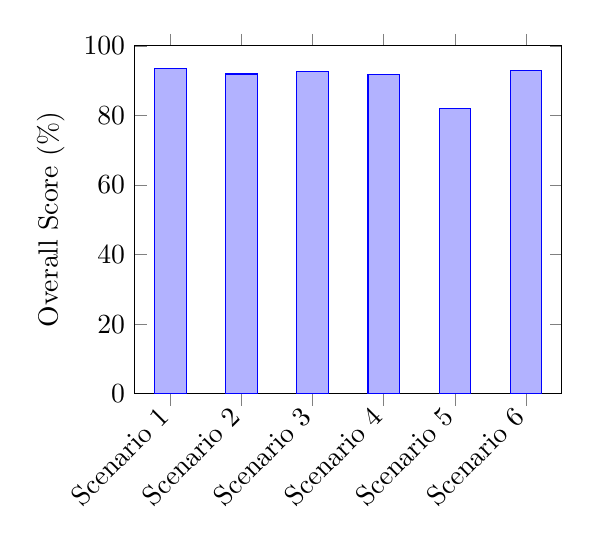
\begin{tikzpicture}
 
    \begin{axis} [ybar,
        height=6cm,
        width=7cm,
        bar width=0.4cm, 
        xlabel={}, 
        ylabel={Overall Score (\%)},
        xtick={1,2,3,4,5,6},
        ymin=0,
        ymax=100,
        xticklabels={Scenario 1,Scenario 2,Scenario 3,Scenario 4,Scenario 5,Scenario 6},
        xlabel style={yshift=-1cm},
            x tick label style={
                rotate=45,
                anchor=east,
            }
        ]
     
     \addplot coordinates {(1,93.6) (2,91.9) (3,92.7) (4,91.8) (5,82.0) (6,92.8)};
     
    \end{axis}
 
    \end{tikzpicture}
    \caption{Mean relative error for each scenario}
    \label{fig:position error}
\end{figure}


Figure \ref{fig:position error} shows the results of this experiment. The system has overall good performance with 5/6 of the scenarios having a relative error of less than 10\%. All scenarios without another MiRo on the pitch showed good accuracy, as well as the scenarios where the ball passed in front of another MiRo. However when the ball passed behind a MiRo and was obscured in scenario 5, the average relative error increased to around 20\%, and there was a much greater variance in accuracy. 

The average score of the system over all six scenarios was 90.8\%, which is accurate enough to be reasonably used in a game of robot football.
 
\subsubsection{Direction and Range Error}

In order to better understand what is causing the error in position, the error can be split into two metrics: direction error and distance error. The direction error represents the difference between the estimated ball position and the MiRo, and the real ball position and the MiRo. The absolute error is used as a higher angle has no impact on the expected accuracy. The distance error represents the error in the estimated distance to the ball compared to the real distance to the ball. 

\begin{figure}[H]
    \centering
    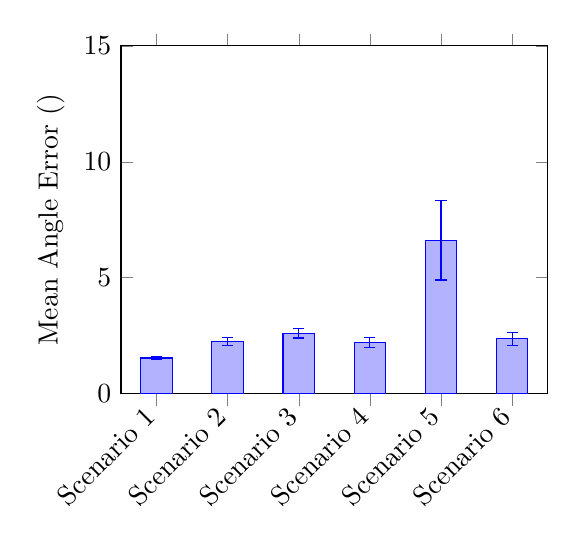
\begin{tikzpicture}
 
    \begin{axis} [ybar,
        height=6cm,
        width=7cm,
        bar width=0.4cm, 
        xlabel={}, 
        ylabel={Mean Angle Error (\degree)},
        xtick={1,2,3,4,5,6},
        ymin=0,
        ymax=15,
        xticklabels={Scenario 1,Scenario 2,Scenario 3,Scenario 4,Scenario 5,Scenario 6},
        xlabel style={yshift=-1cm},
            x tick label style={
                rotate=45,
                anchor=east,
            }
        ]
        
     \addplot+ [
            error bars/.cd,
                y dir=both,
                y explicit relative,
        ] coordinates {
            (1,1.541) +- (0,0.01266*4)
            (2,2.247) +- (0,0.02021*4)
            (3,2.612) +- (0,0.02022*4)
            (4,2.204) +- (0,0.02376*4)
            (5,6.622) +- (0,0.06482*4)
            (6,2.364) +- (0,0.02935*4)
        };
     
    \end{axis}
 
    \end{tikzpicture}
    \hfill
    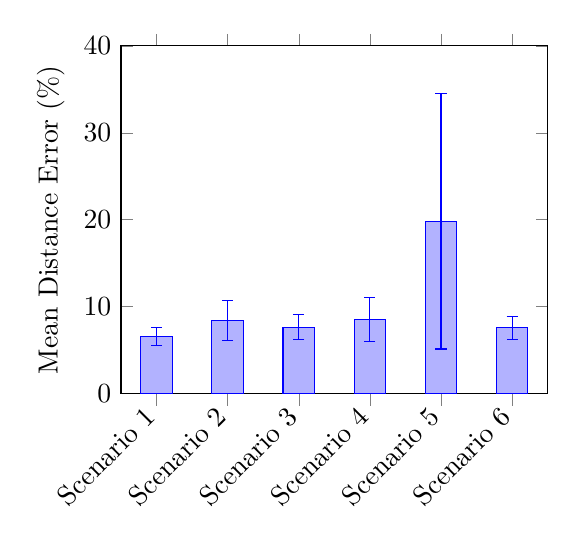
\begin{tikzpicture}
 
    \begin{axis} [ybar,
        height=6cm,
        width=7cm,
        bar width=0.4cm, 
        xlabel={}, 
        ylabel={Mean Distance Error (\%)},
        xtick={1,2,3,4,5,6},
        ymin=0,
        ymax=40,
        xticklabels={Scenario 1,Scenario 2,Scenario 3,Scenario 4,Scenario 5,Scenario 6},
        xlabel style={yshift=-1cm},
            x tick label style={
                rotate=45,
                anchor=east,
            }
        ]
     
     \addplot+ [
            error bars/.cd,
                y dir=both,
                y explicit relative,
        ] coordinates {
            (1,6.577) +- (0,0.04081*4)
            (2,8.409) +- (0,0.06801*4)
            (3,7.649) +- (0,0.04613*4)
            (4,8.514) +- (0,0.07409*4)
            (5,19.848) +- (0,0.1853*4)
            (6,7.564) +- (0,0.04411*4)
        };
     
    \end{axis}
 
    \end{tikzpicture}
    \caption{Mean direction error and relative distance error}
    \label{fig:direction distance error}
\end{figure}

At first glance these results show the same outcome of the previous - that the accuracy is good aside from scenario 5. However looking at the results as a whole, it is clear that the direction error is overall very low with most scenarios having an average error below 3\degree and a small standard deviation, which has a small impact on the relative error of the position. However the average distance error is overall greater and is more often the reason for inaccurate estimations. 

\subsection{Ball Velocity}

To measure the accuracy of the ball velocity estimation, a similar metric to the relative error in the previous section will be used. In order to avoid undefined values when the velocity is zero, a small offset, $a$, will be added to the real velocity. 

\[ \text{Relative error (with offset): } \eta_a =  |1 - \frac{v_{estimate}}{v + a}|\]

\begin{figure}[H]
    \centering
    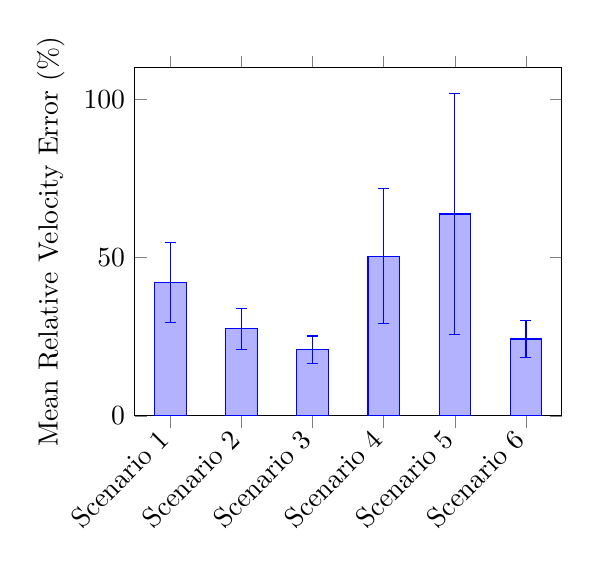
\begin{tikzpicture}
 
    \begin{axis} [ybar,
        height=6cm,
        width=7cm,
        bar width=0.4cm, 
        xlabel={}, 
        ylabel={Mean Relative Velocity Error (\%)},
        xtick={1,2,3,4,5,6},
        ymin=0,
        ymax=110,
        xticklabels={Scenario 1,Scenario 2,Scenario 3,Scenario 4,Scenario 5,Scenario 6},
        xlabel style={yshift=-1cm},
            x tick label style={
                rotate=45,
                anchor=east,
            }
        ]
     
     \addplot+ [
            error bars/.cd,
                y dir=both,
                y explicit relative,
        ] coordinates {
            (1,42.160) +- (0,29.768*0.01)
            (2,27.524) +- (0,23.697*0.01)
            (3,20.945) +- (0,20.499*0.01)
            (4,50.469) +- (0,42.429*0.01)
            (5,63.813) +- (0,59.552*0.01)
            (6,24.277) +- (0,23.994*0.01)
        };
     
    \end{axis}
 
    \end{tikzpicture}
    \caption{Mean relative velocity error for each scenario, $a=1$}
    \label{fig:velocity error}
\end{figure}

These results are interesting as they do not match the the results for the ball position. Scenarios 1 and 4 are considerably less accurate than 2,3 and 6 despite all having similar scores in figure \ref{fig:position error}. One reason for this could be shown in figure \ref{figure: x vs y}, which shows every position estimation that the system made during the scenarios. The estimations for scenarios 2,3 and 6 are all reasonably straight lines, as expected, however the data points for scenarios 1 and 4 form a slight curve, bowing outwards in the centre. This curve seems to be caused by the ball moving both towards and away from the MiRo during these scenarios, showing inaccuracy in the estimation of the distance to the ball. 

\begin{figure}[H]
    \centering
    \includegraphics[width=15cm]{images/x_y.png}
    \caption{Plotting every ball position estimation}
    \label{figure: x vs y}
\end{figure}

\subsection{Ball Trajectory}
\label{section: trajectory results}

In order to measure the accuracy of the ball trajectory prediction, the relative error between the real ball position $t$ seconds in the future and the predicted position at that time is calculated. This means that the last $t$ seconds of each scenario will not be included in the measurement. As the data is collected from the simulation, which does not simulate friction for the ball, the results are expected to be better than in a more realistic situation.

\begin{figure}[H]
    \centering
    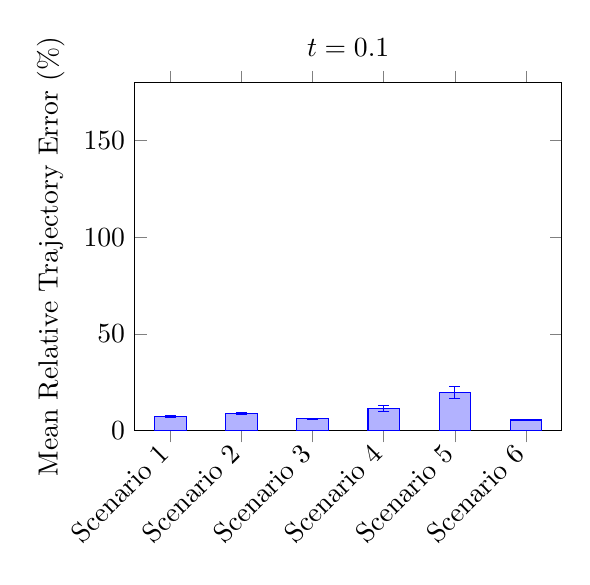
\begin{tikzpicture}
 
    \begin{axis} [ybar,
        title={$t=0.1$},
        height=6cm,
        width=7cm,
        bar width=0.4cm, 
        xlabel={}, 
        ylabel={Mean Relative Trajectory Error (\%)},
        xtick={1,2,3,4,5,6},
        ymin=0,
        ymax=180,
        xticklabels={Scenario 1,Scenario 2,Scenario 3,Scenario 4,Scenario 5,Scenario 6},
        xlabel style={yshift=-1cm},
            x tick label style={
                rotate=45,
                anchor=east,
            }
        ]
     
     \addplot+ [
            error bars/.cd,
                y dir=both,
                y explicit relative,
        ] coordinates {
            (1,7.252) +- (0,5.654*0.01)
            (2,8.828) +- (0,5.940*0.01)
            (3,6.085) +- (0,4.588*0.01)
            (4,11.304) +- (0,13.462*0.01)
            (5,19.822) +- (0,15.417*0.01)
            (6,5.450) +- (0,4.278*0.01)
        };
     
    \end{axis}
 
    \end{tikzpicture}
    \hfill
    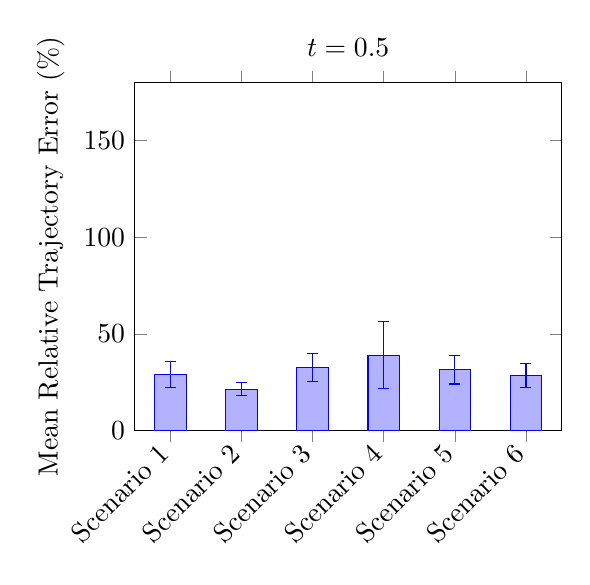
\begin{tikzpicture}
 
    \begin{axis} [ybar,
        title={$t=0.5$},
        height=6cm,
        width=7cm,
        bar width=0.4cm, 
        xlabel={}, 
        ylabel={Mean Relative Trajectory Error (\%)},
        xtick={1,2,3,4,5,6},
        ymin=0,
        ymax=180,
        xticklabels={Scenario 1,Scenario 2,Scenario 3,Scenario 4,Scenario 5,Scenario 6},
        xlabel style={yshift=-1cm},
            x tick label style={
                rotate=45,
                anchor=east,
            }
        ]
     
     \addplot+ [
            error bars/.cd,
                y dir=both,
                y explicit relative,
        ] coordinates {
            (1,29.133) +- (0,22.886*0.01)
            (2,21.425) +- (0,16.319*0.01)
            (3,32.503) +- (0,22.472*0.01)
            (4,38.977) +- (0,44.633*0.01)
            (5,31.541) +- (0,23.690*0.01)
            (6,28.495) +- (0,21.457*0.01)
        };
     
    \end{axis}
 
    \end{tikzpicture}
    
    
    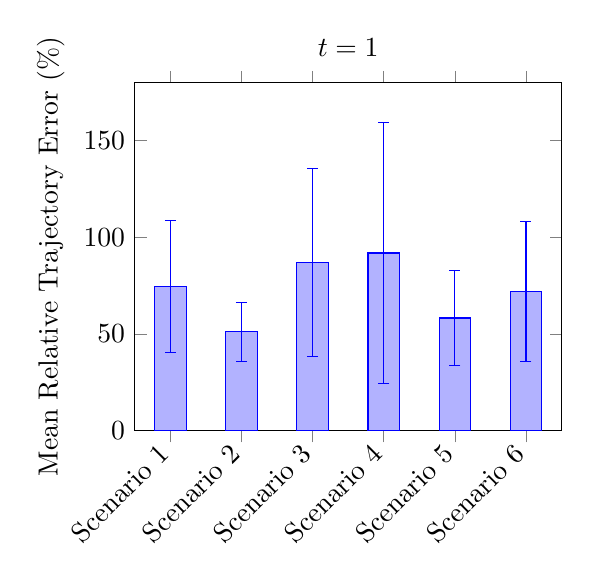
\begin{tikzpicture}
 
    \begin{axis} [ybar,
        title={$t=1$},
        height=6cm,
        width=7cm,
        bar width=0.4cm, 
        xlabel={}, 
        ylabel={Mean Relative Trajectory Error (\%)},
        xtick={1,2,3,4,5,6},
        ymin=0,
        ymax=180,
        xticklabels={Scenario 1,Scenario 2,Scenario 3,Scenario 4,Scenario 5,Scenario 6},
        xlabel style={yshift=-1cm},
            x tick label style={
                rotate=45,
                anchor=east,
            }
        ]
     
     \addplot+ [
            error bars/.cd,
                y dir=both,
                y explicit relative,
        ] coordinates {
            (1,74.725) +- (0,45.689*0.01)
            (2,51.012) +- (0,30.272*0.01)
            (3,87.051) +- (0,55.774*0.01)
            (4,91.819) +- (0,73.479*0.01)
            (5,58.210) +- (0,42.155*0.01)
            (6,71.909) +- (0,50.203*0.01)
        };
     
    \end{axis}
 
    \end{tikzpicture}
    \caption{Mean relative trajectory error for each scenario, $t$ seconds in the future}
    \label{fig:trajectory error}
\end{figure}

When $t = 0.1$, or when the prediction is for the next system iteration, there is already considerable error in the trajectory prediction, especially in scenario 5 which has seen poor results in the previous tests. This inaccuracy grows as $t$ increases, reaching over 100\% error at times when $t$ = 1. These results are not accurate enough to be useful for the game of robot football, particularly because of MiRo's slow speed making it necessary to plan to hit the ball seconds in the future. 

\section{Project Timeline and Objectives Overview}

The aims and objectives from section \ref{section: aims and objectives} are repeated for convenience:
\begin{itemize}
    \item[] \textbf{Essential}
    \item Calibrate MiRo's onboard cameras 
    \item Perform object detection of the ball
    \item Convert from image space to world space
    \item Predict the free movement of the ball
    \item Measure the ball velocity
    \item[] \textbf{Desirable}
    \item Use sensor fusion to improve accuracy
    \item[] \textbf{Optional}
    \item Predict bounces on the trajectory
\end{itemize}

Figure \ref{fig:project timeline} shows the project timeline for the second semester of work, with the deadline during week 11. Some work had been completed before this on a basic system, including the circular Hough transform (\ref{section: Hough design}) and the colour filter (\ref{section: colour filter design}), as well as experiments with the histogram of oriented gradients feature detector (\ref{section: svm-hog}).

\begin{figure}[H]
    \begin{ganttchart}{1}{11}
        \gantttitle{Weeks}{11} \\
        \gantttitlelist{1,...,11}{1} \\
        \ganttgroup{Ball Perception}{1}{5} \\
        \ganttbar{Classifier for HOG Feature}{1}{1} \\
        \ganttbar{Camera Calibration and Image to World Space}{2}{2} \\
        \ganttbar{Local and Global Sensor Fusion}{3}{4} \\
        \ganttbar{Measure Ball Velocity}{5}{5} \\
        \ganttgroup{Ball Trajectory}{6}{8} \\
        \ganttbar{Model for Predicting Trajectory}{6}{7} \\
        \ganttbar{Include Bounces in the Trajectory}{8}{8} \\
    \end{ganttchart}
    \caption{Project timeline}
    \label{fig:project timeline}
\end{figure}

\subsubsection{Camera Calibration}

Camera calibration was a very tricky part of the project to get right, with various different methods being attempted over the weeks. The result of this was a sufficiently accurate calibration, but in order to improve the overall system performance this would be a key area to investigate. 

The objective \textbf{calibrate MiRo's onboard cameras} was successful to a sufficient level for the project, although improvements could be made. 

\subsubsection{Object Detection}

This part of the project went fairly smoothly, with some experiments clearly finding the SVM to be the best classifier to use for the project, however dataset collection proved to be a time-consuming process as thousands of samples had to be manually classified. Some experiments were also done on alternatives to the CHT to reduce reliance on colour data such as sliding window or blob detection, but neither were close to the efficiency of the CHT.

The objective \textbf{Perform object detection of the ball} was successfully met, as the system can efficiently estimate the position of the ball even when there are other MiRos in the vision.

\subsubsection{Converting from Image to World Space}

Although seemingly not too complicated, this part of the project caused some delay due to a systematic error (see \ref{section: image to world}) causing inaccuracies that took quite a lot of time to find the root of. Although this was very time-consuming, it was necessary to accept this delay as the image to world space conversion is such an important part of the system. 

The objective \textbf{convert from image space to world space} was successfully achieved, as shown in the ball position results. Any improvements to this would directly improve the overall performance of the system, although it is not clear how these improvements would be made.

\subsubsection{Sensor Fusion}

A basic local sensor fusion technique was implemented using a Kalman filter which is very useful for combining observations from the left and right cameras, however the scope of this part of the project had to be cut short due the previously discussed delays. 

The objective \textbf{use sensor fusion\ to improve accuracy} was partially met as although no system of robot communication was implemented, a Kalman filter is used to improve accuracy using data from both cameras on one MiRo, which can be extended to include data from other MiRos also. 

\subsubsection{Ball Velocity}

Measuring the ball velocity went well, as a sufficiently accurate solution was implemented within the expected amount of time. Although more time could have been put into experimenting with alternate methods, this would not have been worth it due to the better improvements that could be found elsewhere in the system. 

The objective \textbf{measure the ball velocity} has been successfully met as the system includes a reasonably accurate estimation. 

\subsubsection{Ball Trajectory}

The ball trajectory was a fairly neglected problem due to time constraints near the end of the project, as illustrated by the results (\ref{section: trajectory results}). 

Although a basic solution for predicting ball trajectory has been implemented, the objective \textbf{predict the free movement of the ball} has not been met as the accuracy of this method is not accurate enough to be useful in the game of robot football. Therefore the objective \textbf{predict bounces on the trajectory} has also not been met. 


\begin{table}[H]
\begin{tabular}{l|ccc|}
\cline{2-4}
                                                              & \multicolumn{3}{c|}{Success?}                                \\ \cline{2-4} 
                                                              & \multicolumn{1}{c|}{Yes} & \multicolumn{1}{c|}{Partial} & No \\ \hline
\multicolumn{1}{|l|}{\textbf{Essential}}                      & \multicolumn{3}{l|}{}                                        \\ \hline
\multicolumn{1}{|l|}{Calibrate MiRo’s onboard cameras}        & \multicolumn{1}{c|}{X}   & \multicolumn{1}{c|}{}        &    \\ \hline
\multicolumn{1}{|l|}{Perform object detection of the ball}    & \multicolumn{1}{c|}{X}   & \multicolumn{1}{c|}{}        &    \\ \hline
\multicolumn{1}{|l|}{Convert from image space to world space} & \multicolumn{1}{c|}{X}   & \multicolumn{1}{c|}{}        &    \\ \hline
\multicolumn{1}{|l|}{Predict the free movement of the ball}   & \multicolumn{1}{c|}{}    & \multicolumn{1}{c|}{}        & X  \\ \hline
\multicolumn{1}{|l|}{Measure the ball velocity}               & \multicolumn{1}{c|}{X}   & \multicolumn{1}{c|}{}        &    \\ \hline
\multicolumn{1}{|l|}{\textbf{Desirable}}                      & \multicolumn{3}{l|}{}                                        \\ \hline
\multicolumn{1}{|l|}{Use sensor fusion to improve accuracy}   & \multicolumn{1}{c|}{}    & \multicolumn{1}{c|}{X}       &    \\ \hline
\multicolumn{1}{|l|}{\textbf{Optional}}                       & \multicolumn{3}{l|}{}                                        \\ \hline
\multicolumn{1}{|l|}{Predict bounces on the trajectory}       & \multicolumn{1}{c|}{}    & \multicolumn{1}{c|}{}        & X  \\ \hline
\end{tabular}
\caption{Summary of objectives overview}
\label{tab:objectives overview}
\end{table}

\section{Further work}

There are several key areas that with some further work could improve the system greatly.

\subsection{Camera Calibration}

Any improvements to the camera calibration would provide a direct increase in accuracy of the system. One possible way to improve this would be to experiment with using a circle grid rather than a chessboard, although it is unclear whether this would actually has a positive effect. It could also be beneficial to investigate more closely how the position and rotation in relation to the camera affects the accuracy of the calibration, and how to optimise this process.

\subsection{Feature Extraction}

After some experimentation the circular Hough transform was found to be a good feature extractor due to its computational efficiency, however this forces the system to rely heavily on the colour information of the image. One way that this part of the system could be improved would be to look into online methods of colour segmentation, allowing the system to react to changes in lighting. The other way to solve this problem would be to find more efficient ways to use the geometric information of the image. For example if a more computationally efficient feature descriptor than HOG was found with similar performance for ball detection, a more effective feature extraction algorithm such as sliding window could be used. 

\subsection{Sensor Fusion}

The system currently uses the basic Kalman filter for local sensor fusion, however other more sophisticated versions of the filter such as the extended Kalman filter that have been found to have better performance by teams in RoboCup could be used instead. 

As well as this, global sensor fusion could greatly improve the performance of the system in a real game of robot football, as it would essentially allow a MiRo to see more of the pitch, and even receive information about the ball when it is obscured or too far away to be seen. The fusion of these observations could be implemented by feeding them into the Kalman filter with different process noises representing the confidence of the observation. 
\subsection{Ball Trajectory}

There is lots of room for further work on the ball trajectory algorithm. It would be useful to incorporate forces acting on the ball such as friction in the prediction, as well as investigating how to take bounces against the edge of the pitch into account. More complex mathematical models such as those presented in \ref{section: trajectory lit review} could be experimented with to find a more accurate prediction.

\subsection{Real Life vs Simulation}

Most of the testing for this project was performed in simulation, however it would be useful to evaluate how well the system work in real life as well. For this it would be useful to build a system to more easily obtain real data points for the position of the ball to compare the estimated position. Using an overhead camera, a program could be developed to label recorded video with the position of the ball at each frame, or a ball detection algorithm could be developed without the restriction of needing to run in real time, meaning that more powerful machine learning methods such as a convolutional neural network could be used. 

\subsection{Extending the Scope}

There are various extensions to the project that could build towards a more complete robot football player. 

The first is to build a general ball detector rather than focusing on detecting one specific type of ball. The RoboCup specifications enforce that any ball that is at least 50\% white should be detectable, so this would be a good place to start.

The project could also be extended to a more general vision system for robot football. This would include detecting pitch boundaries, goal posts and other players to gain a fuller idea of the world state. 

Following on from trajectory prediction, a motion planning algorithm could be implemented to allow MiRo to intercept the ball, and could include obstacle avoidance around the other players. 
